\subsection{Translational Controller}
The movements of the quadcopter along the inertial frame directions x, y and z are controlled by the translational controllers. It is decided to structure them as cascade loops, where the velocity and position are controlled in the inner and outer loop respectively. The relation between the controllers is presented in \autoref{fig:cascade}.
%
\begin{figure}[H]
	\centering
	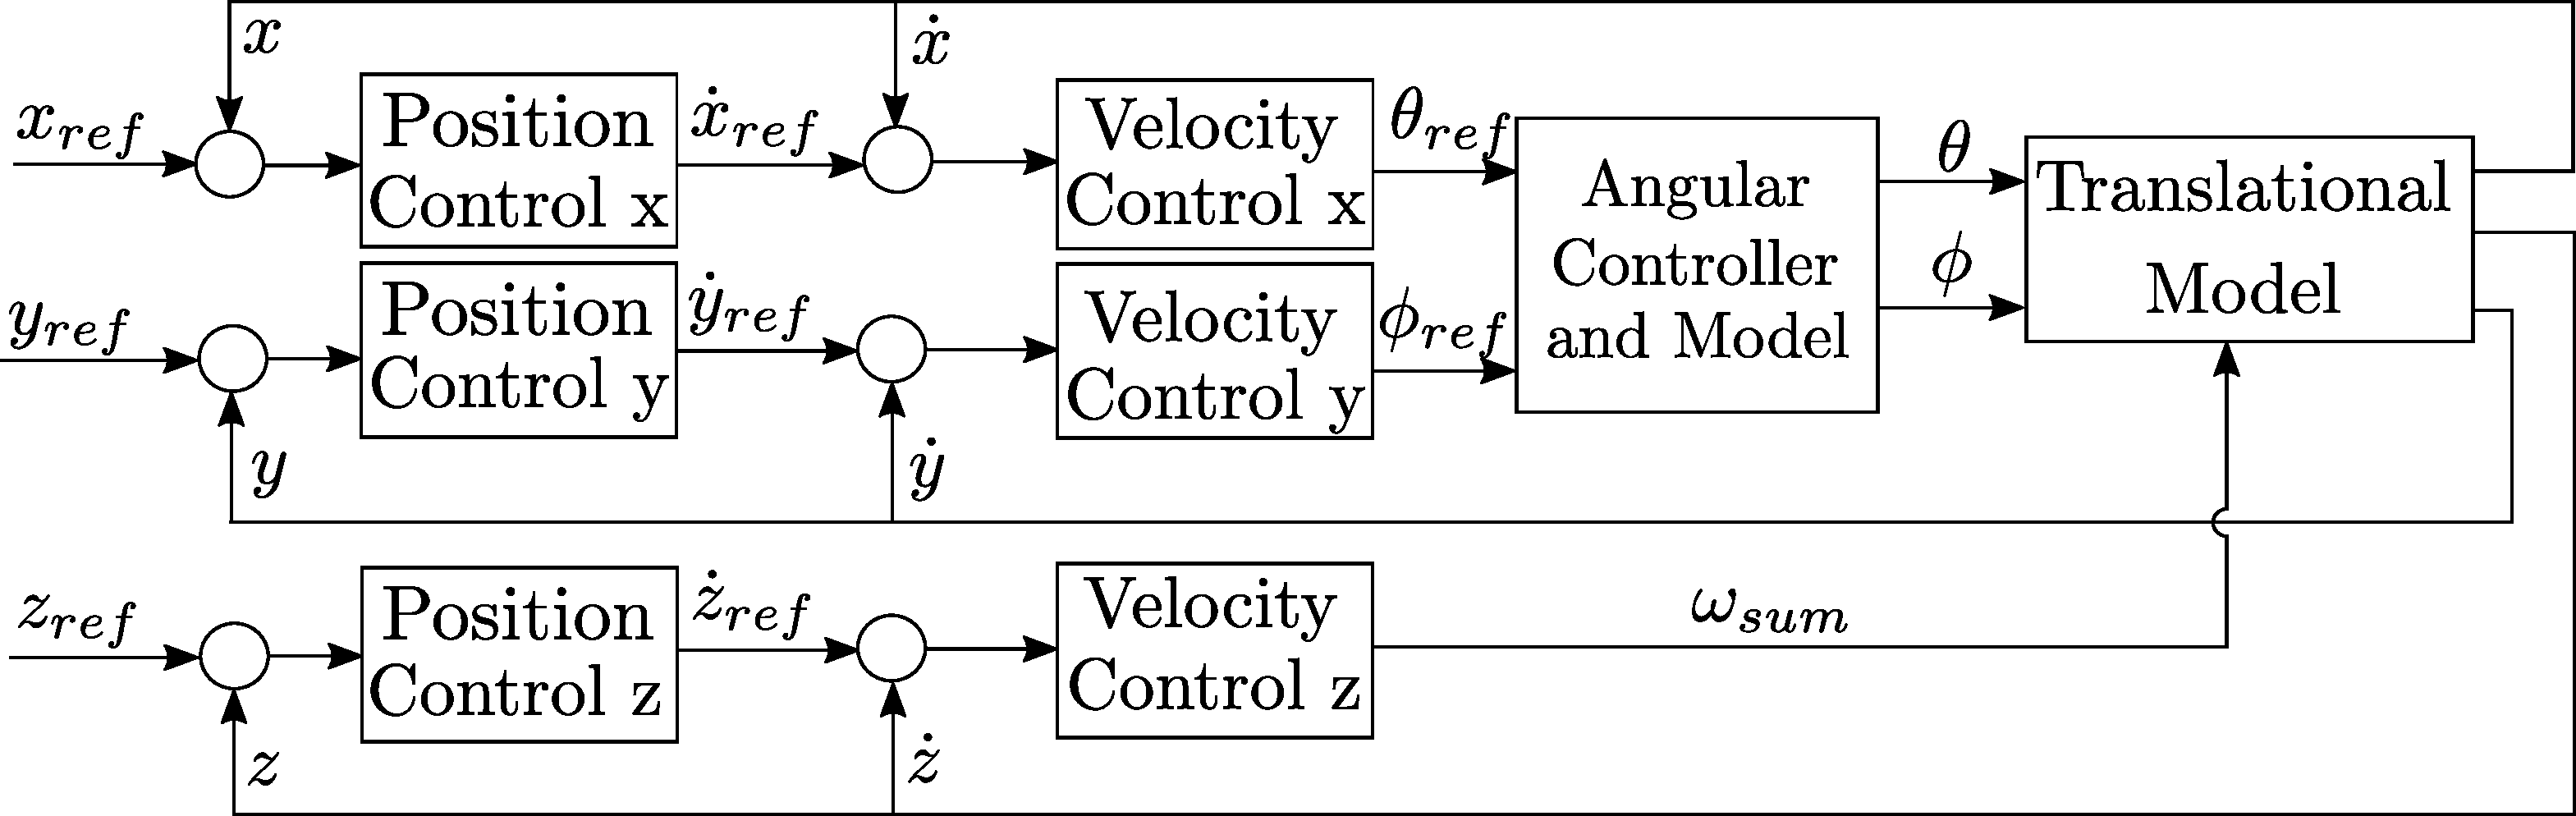
\includegraphics[scale=0.17]{figures/TranslationalControlDiagram.pdf}
	\caption{Overview of control structure.}
	\label{fig:cascade}
\end{figure}

The x and y controller share similar properties as the output for each are an angle reference, $\theta_{ref}$ and $\phi_{ref}$ respectively, while the output of the z controller is the required sum of rotational speeds in the motors.
Firstly the x and y controllers are designed, followed by an individual design for the z controller.\\

To design the inner controllers for x and y velocities, the model equations derived previously, see Equation \ref{eq:AccelerationEqInertial1} and \ref{eq:AccelerationEqInertial2}, are Laplace transformed. They are used to create a transfer function between the angles and the velocities, yielding:
\begin{flalign}
    G_{\dot{x}}(s)&=\frac{\dot{x} (s)}{\theta (s)}=\frac{-k_{th} (\omega_1 ^2 + \omega_2 ^2 + \omega_3 ^2 + \omega_4 ^2)}{m\ s} \\
    G_{\dot{y}}(s)&=\frac{\dot{y} (s)}{\phi (s)}=\frac{k_{th}(\omega_1 ^2 + \omega_2 ^2 + \omega_3 ^2 + \omega_4 ^2)}{m\ s} 
\end{flalign}

Where $G_{x_I}$ and $G_{y_I}$ are the plants used to design the velocity controllers in $x_I$ and $y_I$ direction respectively.

It can be noticed that the plants are the same but with different signs. That is why the controller design is carried out for the x translational velocity and applied to the y translational velocity afterwards.

A proportional controller is considered the plant already has an integrator, that eliminates a steady state error and output disturbances. The gain is the same for both controllers, but must be negative for the x translational controller in order to compensate for its negative plant as this will otherwise be unstable in the closed loop. The gain is designed such that it encounters a bandwidth that is three times lower than the attitude model to ensure minimum effect of disturbances \cite{bandwidthReference}.

The plant of the outer loop is simply an integrator to transform velocity to position. As in the inner loop, the controller of the outer loop is a proportional controller. The outer loop is again designed to have three times less bandwidth than the inner loop to ensure minimization of disturbances and a stable system.\\

To be able to design the inner loop for the z translational controller, the model equation derived previously, see \autoref{eq:AccelerationEqInertial3} is Laplace transformed and written on the form of a transfer function, being the velocity in z direction is the output and the sum of motor rotational speeds is the input.
%
\begin{align}
G_{\dot{z}}=\frac{\dot{z}}{\omega_{sum}} &= \frac{ \frac{1}{4}\ (-2 k_{th})\ \overline{\omega}_{sum} }{ m\ s } & \label{eq:linearTransferFunctionZ}
\end{align}

Where $\dot{z}_I$ is the velocity in the $z_I$ direction, $\omega_{sum}$ is the sum of the rotational speeds of the motors and $\overline{\omega}_{sum}$ is the sum of the rotational speeds in equilibrium.

Due to an integrator and a negative gain the system's locus will move into the right half plane as the gain increases. A proportional controller with negative gain will ensure the system to become stable and to have zero steady state error. However, there are input disturbances given as the equilibrium rotational speeds of the motors maybe be not exactly equal in reality than the calculated ones. In this case, an integrator in the plant is not enough to handle them so another one is added to the controller to eliminate this issue. The final z translational velocity controller results in a  PI-controller. 

As in the case of the x and y outer controllers for position, the plant is just an integrator and, since the disturbances are handled by the inner one, a proportional controller is considered sufficient. This is as well designed so that the bandwidth frequency is three times lower than the inner one.
